\documentclass{llncs}

\usepackage{hyperref}
\usepackage{tikz-cd}
%\usepackage{amsthm}
\usepackage{amsmath}
\usepackage{subfigure}
\usepackage{color}
%\usepackage{comment}
\usepackage{stmaryrd}
\usepackage{listings}
\usepackage{tikz}
\usepackage[all]{xy}
\usepackage{amssymb}
\usepackage{enumerate}

% \lstset{
%   basicstyle={\ttfamily},
%   identifierstyle={\small},
%   commentstyle={\smallitshape},
%   keywordstyle={\small\bfseries},
%   ndkeywordstyle={\small},
%   stringstyle={\small\ttfamily},
%   frame={tb},
%   breaklines=true,
%   columns=[l]{fullflexible},
%   numbers=left,
%   xrightmargin=0zw,
%   xleftmargin=3zw,
%   numberstyle={\scriptsize},
%   stepnumber=1,
%   numbersep=1zw,
%   lineskip=-0.5ex
% }

\newcommand{\Pow}{\mathcal{P}}
\newcommand{\Rel}{\mathrm{Rel}}
\newcommand{\Endo}{\mathrm{Endo}}
\newcommand{\Bidir}{\mathrm{Bidir}}
\newcommand{\Unidir}{\mathrm{Bwd}}
\newcommand{\Bwd}{\mathrm{Bwd}}
\newcommand{\UnidirConst}{\mathrm{BidirConst}}
\newcommand{\Backward}{\mathrm{Backward}}

\newcommand{\tomon}{\to_{\mathrm{mon}}}

\newcommand{\ff}{{f^{\rightarrow}}}
\newcommand{\fb}{{f^{\leftarrow}}}
\newcommand{\gf}{{g^{\rightarrow}}}
\newcommand{\gb}{{g^{\leftarrow}}}
\newcommand{\kf}{{k^{\rightarrow}}}
\newcommand{\kb}{{k^{\leftarrow}}}

\newcommand{\join}{\sqcup}
\newcommand{\bigjoin}{\bigsqcup}
\newcommand{\meet}{\sqcap}
\newcommand{\bigmeet}{\bigsqcap}

\newcommand{\comp}{\circ}
\newcommand{\starlift}{\mathbin{\overline{*}}}
\newcommand{\bowtielift}{\mathbin{\overline{\bowtie}}}
\newcommand{\caplift}{\mathbin{\overline{\cap}}}
\newcommand{\rotleq}{\rotatebox[origin=c]{90}{$\leq$}}
\newcommand{\rotsubseteq}{\rotatebox[origin=c]{90}{$\subseteq$}}
\newcommand{\red}[1]{\textcolor{red}{#1}}
\newcommand{\gray}[1]{\textcolor{gray}{#1}}

\newcommand{\opt}{\mathbf{o}}
\newcommand{\mnd}{\mathbf{m}}
\newcommand{\xs}{\mathit{xs}}

\newcommand{\binop}{\mathtt{binop}}
\newcommand{\binopbw}{\scalebox{0.7}{$\begin{aligned} x,x,\xs &\mapsfrom x, \xs\end\\
\star &\mapsfrom \opt\opt, \star\end{aligned}$}}
\newcommand{\binopfw}{\scalebox{0.7}{$\begin{aligned} \x,x',xs &\mapsto x, \xs\\
                                        \x,\star&\mapsto \star \\
                                      \star &\mapsto \opt,\star\end{aligned}$}}

\newcommand{\push}{\mathtt{push}}
\newcommand{\pushbw}{\scalebox{0.7}{$\begin{aligned} \xs &\mapsfrom x, \xs\end{aligned}$}}
\newcommand{\pushfw}{\scalebox{0.7}{$\begin{aligned} \xs &\mapsto x, \xs \end{aligned}$}}

\newcommand{\load}{\mathtt{load}}
\newcommand{\loadbw}{\scalebox{0.7}{$\begin{aligned} \xs &\mapsfrom x, \xs\end{aligned}$}}
\newcommand{\loadfw}{\scalebox{0.7}{$\begin{aligned} \xs &\mapsto x,\xs \end{aligned}$}}

\newcommand{\dup}{\mathtt{dup}}
\newcommand{\dupbw}{\scalebox{0.7}{$\begin{aligned} \xs &\mapsfrom x, \xs\end{aligned}$}}
\newcommand{\dupfw}{\scalebox{0.7}{$\begin{aligned} \xs &\mapsto x,\xs \end{aligned}$}}

\newcommand{\pop}{\mathtt{pop}}
\newcommand{\popbw}{\scalebox{0.7}{$\begin{aligned} \opt, \xs &\mapsfrom \xs\end{aligned}$}}
\newcommand{\popfw}{\scalebox{0.7}{$\begin{aligned} x, \xs &\mapsto \xs \end{aligned}$}}

\newcommand{\nop}{\mathtt{nop}}
\newcommand{\nopbw}{\scalebox{0.7}{$\begin{aligned} \xs &\mapsfrom \xs\end{aligned}$}}
\newcommand{\nopfw}{\scalebox{0.7}{$\begin{aligned} \xs &\mapsto \xs\end{aligned}$}}

\newcommand{\store}{\mathtt{store}}
\newcommand{\storebw}{\scalebox{0.7}{$\begin{aligned} \mnd, \xs &\mapsfrom \xs\end{aligned}$}}
\newcommand{\storefw}{\scalebox{0.7}{$\begin{aligned} x, \xs &\mapsto \xs\end{aligned}$}}

\newcommand{\print}{\mathtt{print}}
\newcommand{\printbw}{\scalebox{0.7}{$\begin{aligned} \mnd, \xs &\mapsfrom \xs\end{aligned}$}}
\newcommand{\printfw}{\scalebox{0.7}{$\begin{aligned} x, \xs &\mapsto \xs\end{aligned}$}}

\newcommand{\seq}{\mathbin{;}}
\newcommand{\choice}{\mathbin{|}}

\newcommand{\Var}{\mathsf{Var}}
\newcommand{\State}{\mathsf{State}}
\newcommand{\FV}{\mathrm{FV}}

\newcommand{\sqleq}{\sqsubseteq}

\newenvironment{subproof}[1][\proofname]{%
  \renewcommand{\qedsymbol}{$\blacksquare$}%
  \begin{proof}[#1]%
}{%
  \end{proof}%
}




\usetikzlibrary{shapes,arrows}

\tikzstyle{term}=[
  rectangle,
  text width=1.0cm,
  % draw=black,
  %fill=white,
  text centered,
]
\tikzstyle{block}=[
  rectangle,
  text width=1.2cm,
  % draw=black,
  %fill=white,
  text centered,
]

\tikzstyle{arrow}=[
  thick,->,>=stealth
]

\tikzstyle{trans}=[
  thick,=>,>=stealth
]

\tikzstyle{empty}=[
  thick,->,>=stealth
]



\title{Bidirectional data-flow analyses compared to relational through Galois connections}
\author{
  Dylan McDermott
\and
  * Yasuaki Morita
\and
  Tarmo Uustalu
}
\institute{Reykjavik University}
\date{Wed 22 - Thu 23 November NWPT 2023 V{\"a}ster{\aa}s }

\begin{document}
  
\section{Introduction}

\paragraph{Data-flow vs Relational Constraints}
Data-flow analysis
    \begin{itemize}
    \item Many applications in program analysis and compiler optimization.
    \item Information at each program point is propagated over the program by backward or forward transfer \red{functions}.
    \end{itemize}


Constraint-based analysis
    \begin{itemize}
    \item A powerful tool to test property of programs including type inference.
    \item Based on logical formula, equations, and \red{relations}.
    \end{itemize}


\section{Preliminaries}

\subsection{Galois connections}

In this paper, we compare different domains of data-flow analyses in
terms of Galois connections. We need the following basic definitions
and facts.

Given two partial orders $(X, \leq)$, $(Y, \leq)$, a \emph{Galois
  connection} between them is a pair of monotone functions
$\phi : X \to Y$ and $\psi : Y \to X$, called the \emph{lower} and the
\emph{upper adjoint}, such that
\[
\phi(x) \leq y \quad \mathrm{iff} \quad  x \leq \psi(y)
\]
for all $x \in X$, $y \in Y$. Equivalently, one may ask that
\[
x \leq \psi(\phi(x)) \quad \mathrm{and} \quad \phi(\psi(y)) \leq y 
\]
We write $\phi \dashv \psi$ to state this situation.  If
$\phi(\psi(y)) = y$ for all $y \in Y$, the Galois connection is called
a \emph{reflection}. In this case, it $\phi$ is necessarily surjective
and $\psi$ is necessarily injective.

If $\phi \dashv \psi$ is a Galois connection, then all joins
$\bigjoin \{x \mid \phi(x) \leq y\}$ exist, the lower adjoint $\phi$
preserves all joins existing in $X$ and
$\psi(y) = \bigjoin \{x \mid \phi(x) \leq y\}$ (so in particular
$\psi$ is determined by $\phi$). If all joins
$\bigjoin \{x \mid \phi(x) \leq y\}$ exist and are preserved by a
monotone function $\phi : X \to Y$, then $\phi$ is a lower adjoint.

% If both posets $(X, \leq)$ and $(Y, \leq)$ in Galois connection are
% complete lattices, i.e., have joins of all subsets and therefore also
% meets, then the lower adjoint $\phi$ preserves all joins and the upper
% adjoint $\psi$ preserves all meets.  If a monotone function
% $\phi : X \to Y$ preserves all joins, then it is a lower adjoint: the
% upper adjoint is $\psi(y) = \bigjoin \{x \mid phi(x) \leq y\}$.
% Similarly, if a monotone function $\psi : Y \to X$ preserves all
% meets, it is an upper adjoint.

Galois connections are always \emph{idempotent} in that
\[
\psi(y) = \psi(\phi(\psi(y))) \quad \mathrm{and} \quad \phi(\psi(\phi(x))) = \phi(x)
\]  
for all $x \in X$, $y \in Y$.

The set $X_0$ of fixedpoints of $\psi \circ \phi$, i.e., those
elements $x \in X$ for which $x = \psi(\phi(x))$, consists of
precisely the elements of $X$ in the image of $\psi$, i.e., $x$ such
that $x = \psi(y)$ for some $y \in Y$. This set $X_0$ is in a monotone
bijection with the set $Y_0$ of fixedpoints of $\phi \circ \psi$,
i.e., those elements of $y \in Y$ for which $\phi(\psi(y)) = y$. The
set $Y_0$ consists of precisely the elements in the image of $\phi$,
i.e., $y$ such that $\phi(x) = y$.

The monotone bijection between $X_0$ and $Y_0$ is given by the
restrictions of $\phi$ and $\psi$ to $X_0$ and $Y_0$
respectively. Owing to this isomorphism of the posets $(X_0, \leq)$ and
$(Y_0, \leq)$, it is customary to refer to either of them as the poset
of \emph{fixedpoints} of the Galois connection.

If the Galois connection is a reflection, then $Y_0 = Y$. 

Overall, the following picture emerges:
\[
\xymatrix{
(X, \leq) \ar@/^0.5pc/[r]^{\phi} \ar@{}[r]|{\top}
& (Y, \leq) \ar@/^0.5pc/[l]^{\psi}\\   
(X_0, \leq) \ar@{>->}[u] \ar@/^0.5pc/[r]^{\phi|_{X_0}} \ar@{}[r]|{\cong}
& (Y_0, \leq) \ar@{>->}[u] \ar@/^0.5pc/[l]^{\psi|_{Y_0}}
}  
\]

Given a Galois connection $\phi \dashv \psi$ between $(X, \leq)$,
$(Y, \leq)$, we sometimes want to compare two monotone binary
operations ${\otimes} : X \times X \to X$ and
${\boxtimes} : Y \times Y \to Y$. We say that $\boxtimes$
\emph{underapproximates} $\otimes$ if
\[
\psi(y_0 \boxtimes y_1) \leq \psi(y_0) \otimes \psi(y_1) 
\]  
for all $y_0, y_1 \in Y$ and that $\boxtimes$ \emph{overapproximates}
$\otimes$ if
\[
\psi(y_0) \otimes \psi(y_1) \leq \psi(y_0 \boxtimes y_1) 
\]  
Given a monotone binary operation $\otimes : X \times X \to X$, one
can \emph{transport} it to $\bar{\otimes} : Y \times Y \to Y$ defined
by
\[
y_0 \mathbin{\bar{\otimes}} y_1 = \phi(\psi(y_0) \otimes \psi(y_1)) 
\]
The transport $\bar{\otimes}$ is always the least overapproximation of
$\otimes$: it is an overapproximation since
$\psi(y_0) \otimes \psi(y_1) \leq \psi(\phi(\psi(y_0) \otimes
\psi(y_1))) = \psi(y_0 \mathbin{\bar{\otimes}} y_1)$ and it is below
any other overapproximation ${\boxtimes}$ since
$y_0 \mathbin{\bar{\otimes}} y_1 = \phi(\psi(y_0) \otimes \psi(y_1))
\leq \phi(\psi(y_0 \boxtimes y_1)) \leq y_0 \boxtimes y_1$.

\begin{lemma}\label{lem:closedness-lifting-underapproximation}
  The image of $\psi$ is closed under $\otimes$ if and only if the lifting $\bar{\otimes}$ underapproximates $\otimes$.
  \begin{proof}
    Note that the condition on the left hand side is equivalent to $\forall y_{0}, y_{i}. \exists y_{2}. \psi(y_{0}) \otimes \psi (y_{1}) = \psi (y_{2})$.
    It suffices to show that
    \[
      (\exists y. \psi (y) = \psi(y_{0}) \otimes \psi (y_{1}) ) \iff \psi (y_{0} \bar{\otimes} y_{1}) \leq \psi (y_{0}) \otimes \psi (y_{1})
    \]
    for any $y_{0}$ and $y_{1}$.

    Proof of $\impliedby$: Since $\bar{\otimes}$ is an overapproximation of $\otimes$,
    $\psi (y_{0} \bar{\otimes} y_{1}) = \psi (y_{0}) \otimes \psi (y_{1})$ and we give $y_{0} \bar{\otimes} y_{1}$ for $y$

    Proof of $\implies$:
    Define an operation $\boxtimes$ that takes $y_{0}, y_{1}$ and results $y$ such that $\psi(y) = \psi(y_{0}) \otimes \psi(y_{1})$
    Since $\bar{\otimes}$ is the least overapproximation and $\boxtimes$ is an overapproximation (and an underapproximation), we get
    $y_{0} \bar{\otimes} y_{1} \leq y_{0} \boxtimes y_{1} $. Thus, $\psi(y_{0} \bar{\otimes} y_{1}) \leq \psi(y_{0} \boxtimes y_{1}) = \psi(y_{0}) \otimes \psi (y_{1})$
  \end{proof}
\end{lemma}

Underapproximation is harder. If $(Y, \leq)$ has all joins (is a
complete lattice), then one can define
\[
y_0 \mathbin{\underline{\otimes}} y_1 = \bigjoin \{ y \mid \psi(y) \leq \psi(y_0) \otimes \psi(y_1))\} 
\]
$\underline{\otimes}$ is necessarily above all underapproximations of
$\otimes$, but it need not itself be one. However, if $\psi$ preserves
joins (as an upper adjoint it is generally only guaranteed to preserve
meets), then it is the greatest underapproximation of $\otimes$.

There is no general recipe for tgunderapproximation. In general an
operation $\otimes$ may not have any underapproximations at all.

Similar definitions and statements can be made for monotone operations
of any arity, including nullary, i.e., constants.  So, in particular,
we can say that a particular element $y \in Y$ underapproximates
$x \in X$ if $\psi(y) \leq x$ and overapproximates it if
$x \leq \psi(y)$.

The order-theoretic concept of Galois connections is a special case of
adjunctions from category theory and facts about Galois connections
generalize to adjunctions. A Galois connection between two posets is
precisely an adjunction between two thin skeletal categories (there is
at most one map between any two objects and isomorphic objects are
equal). Not every adjunction is idempotent. The fixedpoint theory of
Galois connections generalizes for idempotent adjunctions.


\subsection{Kleene algebras and weaker structures}

We take the view that a programming language, quotiented by semantic
equivalence, is a Kleene algebra (as it supports sequential
composition, nondeterministic choice and iteration obeying the Kleene
algebra equations).

An analysis (of the whole language) will be a homomorphism from this
Kleene algebra to a weaker structure.

A \emph{Kleene algebra} is an idempotent semiring
$(X, 0, {+},1, {\cdot})$ together with a unary operation $(-)^*$ on
$X$ such that $x^*$ is simultaneously the least fixedpoint of both
$1 + x \cdot {-}$ and $1 + {-} \cdot x$.  We note that since
$(X, 0, {+})$ is a idempotent commutative monoid (so an upper
semilattice with bottom), it comes with a partial order given by
$x \leq y$ if $x + y = y$. The operations $+$ and $\cdot$ are both
monotone in both arguments. Therefore, the functions $1 + x \cdot {-}$
and $1 + {-} \cdot x$ are both monotone.

We need to work with a weaker algebraic structure of flow algebras. 

A \emph{flow algebra} is a set $X$ with designated elements $0$, $1$,
binary operations $+$, $\cdot$ and a unary operation $(-)^*$ such that
$(X, 0, {+})$ is an idempotent commutative monoid, $(X, 1, {\cdot})$
is a monoid, $\cdot$ is monotone in both arguments, $(-)^*$ is
monotone and $x^*$ is a prefixedpoint of both $1 + x \cdot {-}$, and
$1 + {-} \cdot x$, i.e.,
\[
  1 + x \cdot x^* \leq x^* \textrm{~and~} 1 + x^* \cdot x \leq x^*  
\]  
Monotonicity of $\cdot$ is equivalent to distributivity of $\cdot$
over $+$ from both the left and the right as an inequation:
\[
  x \cdot y + x \cdot z \leq x \cdot (y+z) \textrm{~and~}
  y \cdot x + z \cdot x \leq (y+z) \cdot x  
\]

A \emph{homomorphism} between flow algebras
$(X, 0, {+}, 1, {\cdot}, (-)^*)$ and
$(Y, 0', {+'}, 1', {\cdot'}, (-)^{*'})$ is a function $h : X \to Y$
that preserves the structure. A \emph{lax homomorphism} is a function
that preserves the structure as inequations:
\[
  0' \leq h(0) \quad h(x) +' h(y) \leq h(x + y) \quad
  1' \leq h(1) \quad h(x) \cdot' h(y) \leq h \cdot (x + y) \quad
  (h(x))*' \leq h(x^*) 
\]  

\section{Unidirectional analyses}

We will now apply Galois connections to study the relationship between
relational and unidirectional (specifically, backward) specification
formats of data-flow analyses---in terms of constraints and backward
transfer functions. We always view the relational specification of an
analysis as its ideal version capturing all semantically valid
analysis results whereas a backward formulation should be a version
tailored to effective computation of the strongest analysis
results. We will explain what we mean by these phrases shortly.

We assume given two complete lattices $(D, \sqleq)$, $(E, \sqleq)$
that could be the data-flow value domains for two program points in a
global program (control-flow graph) connected by a statement
(edge). In usual practice, these domains would be the same for all
program points, but for now we have no reason to restrict
ourselves. They would normally also be assumed to be locally finite
(i.e., with all chains finite), but for now we do not need this
assumption either.

We are interested in the two posets $(\Pow(D \times E), \subseteq)$ and
$(E \tomon D, \sqleq)$ of \emph{binary relations} and \emph{monotone
  backward functions} between $D$ and $E$. We use the elements of
these posets as relational resp.\ backward specifications of data-flow
analyses. For brevity, we also write $\Rel(D, E)$ and $\Bwd(D, E)$
for these two posets. Both are complete lattices in fact; the first
has its joins given by unions, the second by the joins in
$(D, \sqleq)$.

Between these two posets, there is a Galois connection $F \dashv G$
defined by
\begin{align*}
    F (R)(e_{0}) &= \bigjoin \{ d \mid \exists e.\, e \leq e_{0}  \land (d , e) \in R \} \\
    G (\fb) &= \{ (d , e) \mid d \leq \fb(e) \}
\end{align*}

A typical data-flow analysis that we can describe relationally and
backward-unidirectionally is the live variables analysis. Here
$(D, \sqleq) = (E, \sqleq) = (\Pow(\Var), \supseteq)$. For the
assignment statement $x := e$, the transfer function is the monotone
function $\fb (Y) = Y \setminus \{x\} \cup \FV(e)$ (returning the set
of just these variables whose values at the prepoint that can possibly
affect the values of the variables in $Y$ at the postpoint).  The
constraint is $R(X,Y)$ iff $X \supseteq Y \setminus \{x\} \cup \FV(e)$
(accepting any valid pre-post pair of live variable sets in the sense
of noninterference).

It is straightforward to verify that $R = G(\fb)$ and $F(R) = \fb$.  So
$R$ and $\fb$ embody, in $\Rel(D,E)$ resp. $\Bwd(D,E)$, the same
fixedpoint of the Galois connection.

Another archetypical example is preconditions analysis.\footnote{We
  might be more used to think of the preconditions analysis as a
  program logic, but its only ``flaw'' as an analysis is that the
  data-flow value poset is not locally finite.}  Here
$(D, \sqleq) = (E, \sqleq) = (\Pow(\State), \subseteq)$. For the
assignment statement $x := e$, the transfer function is the monotone
function
$\fb (Q) = \{ \sigma \mid \sigma[x \mapsto \llbracket
e\rrbracket(\sigma)] \in Q \}$ (returning the weakest precondition)
while the constraint is the relation $R(P, Q)$ that holds iff
$\forall \sigma.\, \sigma \in P \implies \sigma[x \mapsto \llbracket
e\rrbracket(\sigma)] \in Q$ (accepting any valid pre-postcondition
pair).

In both cases, $\fb = F(R)$, so $\fb$ is the transport of $R$,
therefore the least overapproximation of $R$. Moreover, we also have
$G(\fb) \sqleq R$, so $\fb$ is an underapproximation too. I.e., $\fb$
perfectly agrees with $R$, they are two embodyments, in $\Rel(D,E)$
resp. $\Bwd(D,E)$, of the same fixedpoint of the Galois connection.

We say that a backward-functional specification of analysis is
\emph{sound} if, for any program $s$, the transfer function $\fb_s$
assigned to it underapproximates the constraint $R_s$ assigned to it
by the definitive relational specification, i.e.,
$G(\fb_s) \subseteq R_s$.  For it to be \emph{complete}, $\fb_s$ has
to be an overapproximation of $R$, i.e., $R \subseteq G(\fb_s)$ for
any $s$.

In the two examples we have considered, the transfer function
$\fb$ is both sound and complete wrt.\ the constraint.

For an analysis to admit a sound and complete backward-unidirectional
specification, the constraint for any program must belong to the image
of $G$, i.e., in $\Rel(D,E)_0$.  A relation $R$ turns out to be in the
image of $G$ iff it is \emph{join-closed}, i.e.,
\[
\forall S.\,  S \subseteq R \implies \bigjoin S \in R
\]  
and \emph{pre-down-post-up-closed}, i.e.,
\[
\forall d, e,d_{1 },e_{0}.\, d \leq d_{1} \land e_{0} \leq e \land
(d_{1}, e_{0}) \in R \implies (d, e) \in R
\]
or, pictorially,
\begin{center}
  \begin{tikzcd}
    d_{1} &       \\
    d     & e     \\
          & e_{0}
    \arrow["\rotleq"{name=dd1'}, from=2-1, to=1-1]
    \arrow["\rotleq"{name=e0e'}, from=3-2, to=2-2, swap]
    \arrow[""{name=r10'}, from=1-1, to=3-2, no head]
    \arrow[""{name=r'}, from=2-1, to=2-2, dashed, no head]
  \end{tikzcd}
\end{center}

(Here, we should recognize that the rules of disjunction and
subsumption are valid in Hoare logic.)

(talk about operation liftings)





Notice that our use here of Galois connections to study analyses is
unrelated to the famous one in abstract interpretation where a Galois
connection between a concrete semantics and its abstracted version (a
forward analysis) is given by abstraction and concretization
functions. There, transfer functions are endomaps on the complete
lattice $(D, \sqleq)$ of abstract states. Here, transfer functions are
elements of the complete lattice $(D \tomon D, \sqleq)$ of all
potential transfer function.


\section{Unidirectional analyses}

  \paragraph{Functions and Relations}
  How are they related?
    As a function is a certain kind of a relation,
    a data-flow analysis can be seen as a certain kind of constraint satisfaction problem, or its sound approximation.
    The notion of \emph{Galois connection} consolidates this perspective.
  
  \begin{definition}[Galois connection]
    Given posets $(X, \leq)$ and $(Y, \leq)$, a Galois connection between $(X, \leq)$ , $(Y, \leq)$ is a pair of monotone functions $F : X \tomon Y$ and $G : Y \tomon X$ such that $F(x) \leq y \iff x \leq G(y)$ for all $x \in X$ and $y \in Y$.
    We write this $F \dashv G$.
  \end{definition}

  When $F \dashv G$ is established, the following propositions hold:

  \begin{align}
    F \comp G \comp F = F \\
    G \comp F \comp G = G \\
    x \leq G(F(x)) \\
    F(G(y)) \leq y \\
    \exists y, x = G(y) \implies G(F(x)) = x \\
    \exists x, y = F(x) \implies F(G(y)) = y \\
    F (x \meet y) = F(x) \meet F(y) \\
    G (x \join y) = G(x) \join G (y)
  \end{align}

 \paragraph{A Galois connection in program analysis}

    Consider the poset of all relations (as constraints) on complete lattices, and the poset of monotone functions (as backward transfer functions) on complete lattices.
    The Galois connection $F \dashv G$ is established between them.
  \begin{center}
    \begin{tikzcd}
    (\Pow(D \times E), \subseteq) & = \Rel(D, E) \\
    (E \tomon D, \leq)  & = \Unidir(D, E)
    \arrow["F"{name=left-adj}, bend right=30, swap, from=1-1, to=2-1]
    \arrow["G"{name=right-adj}, bend right=30, swap, from=2-1, to=1-1]
    \arrow["\dashv" rotate=0, phantom, from=left-adj, to=right-adj]
    \end{tikzcd}
  \end{center}
  where $D$ and $E$ are complete lattices of data-flow values corresponding entry and exit point of some program. The left and right adjoint $F$, $G$ are given as follows:
  \begin{align*}
    F(R) &= \lambda e_{0} . \bigjoin \{ d \mid \exists e. e \leq e_{0}  \land (d , e) \in R \} \\
    G(\fb) &= \{ (d , e) \mid d \leq \fb(e) \} \\
  \end{align*}

  Explicitly, $F \comp G$ and $G \comp F$ are presented as follows:
  \begin{align*}
    G(F(R)) &= \{ (d_{0},e_{0}) \mid d_{0} \leq \bigjoin \{ d \mid \exists e.e \leq e_{0} \land (d,e) \in R \}\} \\
    F(G(\fb)) &= \lambda e_{0} . \bigjoin \{ d \mid \exists e. e \leq e_{0} \land d \leq \fb(e) \} = \fb
  \end{align*}

\paragraph{The class of relations via the Galois connection}
  The image of $G$ is the class of relations that can be specified by backward transfer functions.
  This class of relations is equivalent to the condition being a fixed point of the Galois connection i.e., a relation $R$ satisfies $G(F(R)) = R$. Since any relation is a postfixed point ($R \subseteq G(F(R))$) by nature of Galois connections, the class of relations also equivalent to the condition of relation $R$ being a prefixed point $G(F(R)) \subseteq R$.
  We obtain the characterization of the class from general facts about Galois connection:
  \begin{proposition}\label{prop:predown-postup}
  $R$ is in the image of $G$ if and only if $R$ is $\join$-closed and $R$ is pre-down-/post-upclosed,
  where $R$ is pre-down-/post-upclosed if and only if the condition
  \begin{align*}
  \forall d, e, d_{1 }, e_{0}. d \leq d_{1} \land e_{0} \leq e \land (d_{1}, e_{0}) \in R \implies (d, e) \in R
  \end{align*}
  is met.
  The following diagram represents pre-down-/post-upclosedness:
  \begin{center}
  \begin{tikzcd}
    d_{1} &       \\
    d     & e     \\
          & e_{0}
    \arrow["\rotleq"{name=dd1'}, from=2-1, to=1-1]
    \arrow["\rotleq"{name=e0e'}, from=3-2, to=2-2, swap]
    \arrow[""{name=r10'}, from=1-1, to=3-2, no head]
    \arrow[""{name=r'}, from=2-1, to=2-2, dashed, no head]
  \end{tikzcd}
  \end{center}
  \end{proposition}


  \begin{example}
    The pre-down-/post-upclosed condition fits in pre-condition weakening and post-condition strengthening in Hoare logic: $L$ is for a set of live variables and the order $\leq$ is the set inclusion $\supseteq$.
    For example, a triple $\{ L \backslash \{ x \} \} x = 10 \{ L \}$ is valid (relation is functional but the logic is still valid when replacing precondition with any $L' \supseteq L \{ x \}$ and postcondition with any $L'' \subseteq L$.
  \end{example}

  Note that the image of $F$, equivalently the fixedpoint of $F \comp G$, coinsides $\Unidir(D , E)$ itself. This follows from $F (G (\fb))) = \fb$.

  We introduce \emph{completeness} and \emph{soundness} for operations on functions with regard to some operation on relations.
  \begin{definition}[Completeness]
   A binary operation $\otimes$ on backward transfer functions is \emph{complete} with regard to $*$ on binary operation on relations if and only if for every relation $R \in G(\fb) * G(\gb)$, $R$ is also $G (\fb \otimes \gb)$, i.e., $G(\fb) * G(\gb) \subseteq G (\fb \otimes \gb)$.
  \end{definition}

  \begin{definition}[Soundness]
  A binary operation $\otimes$ on backward transfer functions is \emph{sound} with regard to $*$ on binary operation on relations if and only if
  $G (\fb \otimes \gb) \subseteq G(\fb) * G(\gb)$
  \end{definition}

  \paragraph{Operation Lifting}
  For a given binary operation $*$ on relations, a lifted binary operation $\starlift$ on backward transfer functions can be obtained by $F \dashv G$ as follows:
  \begin{align*}
  \fb \starlift \gb = F (G(\fb) * G(\gb))
  \end{align*}
  Any lifted operation $\starlift$ is complete with regard to $*$:
  \begin{align*}
  G(\fb) * G(\gb) \subseteq G(F(G(\fb) * G(\gb))) = G(\fb \starlift \gb)
  \end{align*}


\paragraph{Composition lifting via Galois connection}


  Sequencing of constraints
    The constraint corresponds to the sequential composition is the relational composition $\bowtie$ of the constraints of first and second pieces of code.
f
    By using $F \dashv G$, the lifted composition of transfer functions $\bowtielift$ is obtained, which is identical to the ordinary function composition $\comp$ in the end.
    \begin{align*}
      \cdot \bowtielift \cdot &: \left| \Unidir(C, D) \right| \times  \left| \Unidir(D, E) \right| \to  \left| \Unidir(C, E) \right| \\
      (\fb \bowtielift \gb) (e_{0}) &= F(G(\fb) \bowtie G(\gb)) (e_{0}) \\
                                  &= \bigjoin \{ c \mid \exists d\, e.\,e \leq e_{0} \land c \leq \fb(d) \land d \leq \gb(e) \} \\
                                  &= \pi_{1} (\bigjoin \{ (c, d , e) \mid e \leq e_{0} \land c \leq \fb(d) \land d \leq \gb(e) \}) \\
                                  &= (\fb \comp \gb)(e_{0})
    \end{align*}
    \begin{proposition}\label{prop:backword-closed-under-composition}
      The image of $G$ is closed under $\bowtie$.
      \begin{proof}
        Leveraging Lemma \ref{lem:closedness-lifting-underapproximation}, the proposition is equivalent to the condition $\bowtielift$ underapproximates $\bowtie$, which means:
        \[
          c \leq \fb (\gb (e)) \implies \exists d. c \leq \fb(d) \land d \leq \gb(e).
        \] for any $c$ and $e$.
        In fact, if $c \leq \fb (\gb (e))$ then $c \leq \fb(d)$ and $d \leq \gb(e)$ is true when $d = \gb(e)$. Thus, $\bowtielift$ underapproximates $\bowtie$, and the image of $G$ is closed under $\bowtie$. \qed
      \end{proof}
    \end{proposition}
  \paragraph{Composition lifting via Galois connection}

  Non-deterministic choice of constraints
    The constraint corresponding to the non-deterministic choice of programs is the intersection $\cap$ of choices.
 Lifting of composition in poset of backward transfer functions
    Similarly to the sequential composition, we get choice operation $\caplift$ on backward transfer functions which is identical to $\meet$ pointwisely.
    \begin{align*}
      \cdot \caplift \cdot &: \left| \Unidir(D , E) \right| \times  \left| \Unidir(D, E) \right| \to \left| \Unidir(D, E) \right| \\
      (\fb \caplift \gb) (e_{0})
      &= F(G(\fb) \cap G(\gb)) (e_{0}) \\
      &= F(G(\fb \meet \gb)) (e_{0}) \\
      &= \bigjoin \{ d \mid \exists e\,. e \leq e_{0} \land d \leq \fb(e) \meet \gb(e) \} \\
      &= \fb(e_{0}) \meet \gb(e_{0})
    \end{align*}

    We can see that taking meet of backward functions gives us ideal approximation for non-deterministic choice within the image of $G$:
    \begin{proposition}\label{prop:backword-closed-under-intersection}
      The image of $G$ is closed under $\cap$.
      \begin{proof}
        Recall that $\cap$ is meet in $\Rel(D , E)$ and the upper adjoint $G$ preserves all meets.
        Consider two relations that can be represented by $G(\fb)$ and $G(\gb)$.
        Since $G$ preserves meets, the intersection $G(\fb) \cap G(\gb)$ is equals to $G(\fb \meet \gb)$. Therefore, the image of $G$ is closed under $\cap$.
      \end{proof}
    \end{proposition}
    Notice that the above proof only relies on the fact $G$ being an upper adjoint.
    The above result can be generalized to any upper adjoint to $\Rel(D \times E)$ from a poset with binary meets:

    \begin{lemma}\label{lem:any-fixedpoint-of-galois-connection-closed-under-intersection}
      Let $(Y, \leq)$ be a poset with binary meets and $\psi : (Y , \leq) \to \Rel(D, E)$ be an upper adjoint.
      Then the image of $\psi$ is closed under $\cap$.
      \begin{proof}
        $\psi(y_{0}) \cap \psi(y_{1}) = \psi(y_{0} \meet y_{1})$
      \end{proof}
    \end{lemma}

  \paragraph{Soundness and Completeness}
  Propositions \ref{prop:backword-closed-under-composition} and \ref{prop:backword-closed-under-intersection} validates the soundness of backward (and forward, by symmetry) data-flow analysis within the image of $G$.  This illustrates how the algorithm for data-flow analysis work:

  Example: Live variable analysis
   \begin{center}
  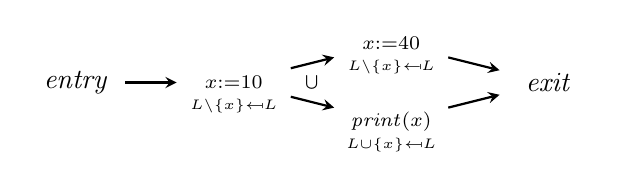
\begin{tikzpicture}[auto]
    \node[term] at (0, 0.0) (entry) {\emph{entry}};
    \node[block] at (2, 0.0) (s1) {$\scriptstyle{x := 10}$};
    \node[block] at (4, 0.5) (s2)   {$\scriptstyle{x := 40}$};
    \node[block] at (4, -0.5) (s3)   {$\scriptstyle{\mathit{print}(x)}$};
    \node[term] at (6, 0.0) (exit)  {\emph{exit}};
    \draw [arrow] (entry) -- (s1);
    \draw [arrow] (s1) -- (s2);
    \draw [arrow] (s1) -- (s3);
    \draw [arrow] (s3) -- (exit);
    \draw [arrow] (s2) -- (exit);
    \node[block] at (2, -0.3) (load0) {$\scriptscriptstyle{L \setminus \{ x \} \mapsfrom L }$};
    \node[block] at (3, 0) (entry) {$\scriptscriptstyle{\bigcup}$};
    \node[block] at (4, 0.2) (pop)   {$\scriptscriptstyle{L \setminus \{ x \} \mapsfrom L }$};
    \node[block] at (4, -0.8) (store)   {$\scriptscriptstyle{L \cup \{ x \} \mapsfrom L}$};
  \end{tikzpicture}
  \end{center}

  where the domain of data-flow values is a set of live variables $\{\emptyset, \{ x \}\}$, and $\meet$ is the set union $\cup$.

\section{Bidirectional data-flow analyses}  

  \paragraph{Bidirectional Data-Flow Analysis}
  Sometimes, analyzing data-flow in both backward and forward directions is necessary. This is known as \emph{bidirectional data-flow analysis}.

  Examples
  \begin{itemize}
    \item Partial redundancy elimination
    \item Type inference for a dynamically typed language
    \item Load-pop pair elimination for stack-based language
  \end{itemize}
  Based on our insights from the unidirectional analysis, it make sense to investigate the Galois connection, the associated class of relations, and the behavior of program compositions in the context of bidirectional data-flow analysis.

  \paragraph{The Galois Connection for Bidirectional Transfer Functions}
  The Galois connections $H \dashv I$ , $J \dashv K$ and $P \dashv M$ are established among the relational constraints, endo monotone functions on product lattice, the bidirectional transfer functions, and the backward unidirectional functions. These factor through $F \dashv G$ by $(P \comp J \comp H) \dashv (I \comp K \comp M)$.
  \begin{center}
    \begin{tikzcd}
      (\Pow(D \times E), \subseteq) & = \Rel(D, E) \\
      ((D \times E) \tomon (D \times E) , \leq) & = \Endo(D, E) \\
      ((E \tomon D) \times (D \tomon E) , \leq) & = \Bidir(D, E) \\
      (E \tomon D , \leq) & = \Unidir(D, E)
        \arrow["H"{name=H}, bend right=30, swap, from=1-1, to=2-1]
        \arrow["I"{name=I}, bend right=30, swap, from=2-1, to=1-1]
        \arrow["J"{name=J}, bend right=30, swap, from=2-1, to=3-1]
        \arrow["K"{name=K}, bend right=30, swap, hook, from=3-1, to=2-1]
        \arrow["P"{name=P}, bend right=30, swap, from=3-1, to=4-1]
        \arrow["M"{name=M}, bend right=30, swap, hook, from=4-1, to=3-1]
        \arrow["\dashv", phantom, from=H, to=I]
        \arrow["\dashv", phantom, from=J, to=K]
        \arrow["\dashv", phantom, from=P, to=M]
    \end{tikzcd}
  \end{center}
  The monotone functions consists of the Galois connections are given as follows:
  \begin{align*}
    H &: \Rel \tomon \Endo &
    I &: \Endo \tomon \Rel \\
    H(R) &= \lambda p_{0} . \bigjoin (\downarrow p_{0} \cap R) &
    I(f) &= \{p \mid p \leq f(p)\} \\
    J &: \Endo \tomon \Bidir &
    K &: \Bidir \tomon \Endo \\
    J(f) &= (\lambda e . \pi_{1} (f (\top , e )) , \lambda d . \pi_{2} (f (d , \top))) &
    K(\fb , \ff) &= \lambda (d , e) . (\fb(e) , \ff(d)) \\
    P &: \Bidir \tomon \Unidir &
    M &: \Unidir \tomon \Bidir \\
    P(\fb , \ff) &= \fb &
    M(\fb) &= (\fb , \top)
  \end{align*}

  \subsection{The Class of Relations for Endomonotone Functions -- $\join$-closed}
  The image of $I$, i.e., all prefixed-points of $I \comp H$, is characterized by $\join$-closedness:
  \begin{theorem}\label{thm:join-closed}
    A relation $R$ is in the image of $I$ if and only if $R$ is $\join$ \text{-closed}
  \end{theorem}

  By pre-composing with some monotone function to $I$, the image becomes more restricted.
  \begin{proposition} \label{prop:restriction-subset}
    Given any monotone function $I'$ whose codomain is $\Endo(D, E)$, the image of $I \comp I'$ is included by the image of $I$.
    Hence, if a relation $R$ is in the image of $I \comp I'$ then $R$ is $\join$-closed.
  \end{proposition}
  Specifically, all relations in the image of $I \comp K$ and of $I \comp K \comp M$ are $\join$-closed.

  The image of $H$, i.e., all postfixed points of $H \comp I$, is characterized by being interior operator:
  \begin{proposition}\label{prop:interior-op}
  $f$ is in the image of $F$ if and only if $f$ is an interior operator,
  where $f$ is interior operator if and only if $f$ satisfies the following condition
  \begin{align*}
    f(e) \leq  e \sqcap f (f (e)).
  \end{align*}
  \end{proposition}

  We can see that the image of $I$ is closed under both $\bowtie$ and $\cap$ which implies $\bowtielift$ and $\caplift$ made from $H \vdash I$ underapproximates $\bowtie$ and $\cap$, respectively.
  \begin{proposition}\label{prop:endo-closed-under-composition}
    The image of $I$ is closed under $\bowtie$.
  \end{proposition}
  \begin{proposition}\label{prop:endo-closed-under-intersection}
    The image of $I$ is closed under $\cap$.
    \begin{proof}
      Since $I$ is an upper adjoint, it follows from Lemma \ref{lem:any-fixedpoint-of-galois-connection-closed-under-intersection}.
    \end{proof}
  \end{proposition}


  % we need to add Endo condition
  % expansion of lifting
  % expansion of composition of H I. etc
  \subsection{The Class of Relations for Bidirectional Flow -- Butterfly}
  The image of $I \comp K$, the class of relations represented by a bidirectional function pair, is characterized as follows

  \begin{proposition}\label{prop:butterfly}
    $R$ is in the image of $I \comp K$ if and only if $R$ is $\join$-closed and has a property called \emph{butterfly}.
  \end{proposition}
  \begin{definition}[Butterfly relation]
    A relation $R$ is \emph{butterfly} if and only if \begin{align*}
      &\forall d, e, d_{0}, d_{1 }, e_{0}, e_{1} .
      d_{0} \leq d \leq d_{1} \land e_{0} \leq e \leq e_{1} \land (d_{1}, e_{0}) \in R \land (d_{0}, e_{1}) \in R \implies (d, e) \in R,
    \end{align*}or diagramatically, \quad
  \begin{tikzcd}
    d_{1} & e_{1} \\
    d     & e     \\
    d_{0} & e_{0}
    \arrow["\rotleq"{name=d0d'}, from=3-1, to=2-1]
    \arrow["\rotleq"{name=dd1'}, from=2-1, to=1-1]
    \arrow["\rotleq"{name=ee1'}, from=2-2, to=1-2, swap]
    \arrow["\rotleq"{name=e0e'}, from=3-2, to=2-2, swap]
    \arrow[""{name=r01'}, from=3-1, to=1-2, no head]
    \arrow[""{name=r10'}, from=1-1, to=3-2, no head]
    \arrow[""{name=r'}, from=2-1, to=2-2, dashed, no head]
  \end{tikzcd}
  \end{definition}

  The image of $J \comp H$, the class of pairs of monotone functions that are fixed points of $J \comp H \comp I \comp K$ is characterized as follows:
  \begin{proposition} \label{prop:pair-nice}
    A pair of function $(\fb , \ff)$ is in the image of $J \comp H$ if and only if $\fb$ and $\ff$ satisfy the following conditions:
    \begin{enumerate}[i.]
      \item $\fb(e) \leq \fb(e \meet \ff (\fb(e)))$
      \item $\ff(d) \leq \ff(d \meet \fb (\ff(d)))$
    \end{enumerate}
  \end{proposition}
  \paragraph{Composition and Butterfly property -- A Case of Failure}

  The \emph{butterfly} relations nicely behave with non-deterministic choice.
  \begin{proposition}
    The image of $J \comp H$ is closed under $\cap$
  \end{proposition}
  However, it does not for sequential composition:
  \begin{proposition}
    The image of $J \comp H$ is not closed under $\bowtie$

    \begin{example}
      The following two butterfly relations $R$ and $S$ are examples where their composition $R \bowtie S$ does not result in a butterfly relation.
      \begin{center}
        \begin{tikzcd}
              &      \\
              & d_{1}\\
        c_{0} & d_{0}
        \arrow["\rotleq"{name=d0d1}, from=3-2, to=2-2, swap]
        \arrow["R"{name=r00}, from=3-1, to=3-2, no head, swap]
        \arrow["R"{name=r01}, from=3-1, to=2-2, no head]
        \end{tikzcd}
        $\bowtie$
        \begin{tikzcd}
              & e_{2} \\
        d_{1} & e_{1} \\
        d_{0} & e_{0}
        \arrow["\rotleq"{name=d0d1'}, from=3-1, to=2-1]
        \arrow["S"{name=s00}, from=3-1, to=3-2, no head, swap]
        \arrow["S"{name=s01}, from=2-1, to=1-2, no head]
        \arrow["\rotleq"{name=e0e1'}, from=3-2, to=2-2, swap]
        \arrow["\rotleq"{name=e1e2'}, from=2-2, to=1-2, swap]
        \end{tikzcd}
        $\quad=\quad$
        \begin{tikzcd}
              & e_{2} \\
              & e_{1} \\
        c_{0} & e_{0}
        \arrow["R \bowtie S"{name=rs0}, from=3-1, to=3-2, no head, swap]
        \arrow["/" marking, from=3-1, to=2-2, dashed, no head, gray]
        \arrow["R \bowtie S"{name=rs1}, from=3-1, to=1-2, no head]
        \arrow["\rotleq"{name=e0e1'}, from=3-2, to=2-2, swap]
        \arrow["\rotleq"{name=e1e2'}, from=2-2, to=1-2, swap]
        \end{tikzcd}
      \end{center}
      Not having the gray dashed line violates being butterfly.
    \end{example}
  \end{proposition}

  Thus, while we can explicitly give a sequencing operation in bidirectional functions by lifting, i.e.,
  \begin{equation*}
    (\fb,\ff) \bowtielift (\gb,\gf) = I(H((\fb, \ff)) \bowtie H((\gb , \gf))),
  \end{equation*}
  the outcome is only guaranteed to be an overapproximation and it may not be sound (underapproximation).

  In the context of analysis of load-pop pairs for stack-based language,
  we have found the case: The sequential composition $\binop; \pop$ is not butterfly while both $\binop$ and $\pop$ are butterfly.
  \begin{figure}
  \begin{tikzcd}[column sep=tiny]
               & \opt,\opt,xs & \quad &          \\
  \opt,\mnd,xs & \mnd,\opt,xs & & \opt, xs \\
               & \mnd,\mnd,xs & & \mnd, xs
  \arrow["\leq", from=3-2, to=2-1, swap, sloped]
  \arrow["\leq", from=3-2, to=2-2, swap, sloped]
  \arrow["\leq", from=2-1, to=1-2, sloped]
  \arrow["\leq", from=2-2, to=1-2, sloped]
  \arrow["\leq", from=3-4, to=2-4, sloped]
  \arrow["", from=3-2, to=3-4, no head, swap]
  \arrow["", from=1-2, to=2-4, no head, swap]
  \end{tikzcd}
  \begin{tikzcd}[column sep=tiny, row sep=small]
           & \quad & \\
  \opt, xs & & \\
  \mnd, xs & & xs
  \arrow["\leq", from=3-1, to=2-1, swap, sloped]
  \arrow["", from=3-1, to=3-3, no head, swap]
  \arrow["", from=2-1, to=3-3, no head, swap]
  \end{tikzcd}
  \caption{The constraints for the instructions $\binop$ (left) and $\pop$ (right)}
  \end{figure}

  \begin{figure}
  \begin{tikzcd}[column sep=tiny, row sep=small]
               & \opt,\opt,xs & \quad &          \\
  \opt,\mnd,xs & \mnd,\opt,xs & &          \\
               & \mnd,\mnd,xs & & xs
  \arrow["\leq", from=3-2, to=2-1, swap, sloped]
  \arrow["\leq", from=3-2, to=2-2, swap, sloped]
  \arrow["\leq", from=2-1, to=1-2, sloped]
  \arrow["\leq", from=2-2, to=1-2, sloped]
  \arrow["", from=3-2, to=3-4, no head, swap]
  \arrow["", from=1-2, to=3-4, no head, swap]
  \end{tikzcd}
  \caption{The constraint for $\binop;\pop$, missing gray lines violates butterfly}
  \end{figure}

  \paragraph{Implications for Bidirectional Flow Analysis}
  A sequence of instructions $i_{1};i_{2}\cdots;i_{n}$ without any branch in/out except for entry/exit is called a \emph{basic block}.


  In Unidirectional Flow Analysis
    Traditionally, each basic block in a program is treated as a single node in the flow graph.
 
  In Bidirectional Flow Analysis
    \red{Cannot} put a basic block into a single node naively.

  This is because composition of two bidirectional function pairs would introduce constraint that is not captured by a single bidirectional function pair. Treating each instruction as an individual node is a safe option but has drawbacks in terms of the efficiency of the analysis.


%    In traditional data-flow analysis, we use basic blocks as building blocks. A basic block is a sequence of instructions with only one entry and one exit. In unidirectional analysis, we can usually put these sequence together into a single node in the flow graph. But, in bidirectional analysis, we cannot do so naively because the composition of two bidirectional function pair would introduce constraints that is not captured by single bidirectional function pair.

% 
%  \paragraph{Solution 1 -- $n$-tupling}
%  A simple solution to this is to stop consolidating basic blocks into a single node and instead treat each instruction as one node.

%   In this approach, the constraints arise from a basic block consists of $n-1$ instructions are treated as an element of $n$-ary relations $\Pow(D_{1} \times D_{2} \times  \cdots  \times D_{n})$, and within the basic block, the carriers of data flow values become $(n-1)$-tuples of pairs of monotone functions $((D_{1} \tomon D_{2}) \times (D_{2} \tomon D_{1}) \times \cdots \times (D_{n-1} \tomon D_{n}) \times (D_{n} \tomon D_{n-1}))$.
%
%   The soundness of lifted operations still holds for the Galois connection between those posets but compositionality is somewhat broken in that intermediate program points cannot be hidden in sequential composition.
% 

  \paragraph{A Remedy -- Narrowing the class of relations }
  The poset of $((E \tomon D) \times E, \leq) = \UnidirConst(D, E)$ locates between $\Bidir(D , E)$ and $\Unidir(D , E)$.
  The Galois connection $P' \dashv M'$ and $ P'' \dashv M''$ is established and factors $P \dashv M = (P'' \comp P') \dashv (M' \comp M'')$.
  \begin{center}
    \begin{tikzcd}
      (\Pow(D \times E), \subseteq) & = \Rel(D, E) \\
      ((E \tomon D) \times (D \tomon E) , \leq) & = \Bidir(D, E) \\
      ((E \tomon D) \times E, \leq) & = \UnidirConst(D, E) \\
      (E \tomon D , \leq) & = \Unidir(D, E)
        \arrow["J \comp H"{name=H}, bend right=30, swap, from=1-1, to=2-1]
        \arrow["I \comp K"{name=I}, bend right=30, swap, from=2-1, to=1-1]
        \arrow["P'"{name=J}, bend right=30, swap, from=2-1, to=3-1]
        \arrow["M'"{name=K}, bend right=30, swap, hook, from=3-1, to=2-1]
        \arrow["P''"{name=M}, bend right=30, swap, from=3-1, to=4-1]
        \arrow["M''"{name=N}, bend right=30, swap, hook, from=4-1, to=3-1]
        \arrow["\dashv", phantom, from=H, to=I]
        \arrow["\dashv", phantom, from=J, to=K]
        \arrow["\dashv", phantom, from=M, to=N]
    \end{tikzcd}
  \end{center}
  where
  \begin{align*}
    P'(\fb , \ff) &= (\fb , \ff(\top)) & M'(\fb , k) &= (\fb , \lambda d. k) \\
    P''(\fb , e) &= \fb & M''(\fb) &= (\fb , \top)
  \end{align*}

  Indeed, the class of relations corresponds to the Galois connection between $\Rel(D, E)$ and $\UnidirConst(D, E)$ is closed under both $\cap$ and $\bowtie$.

  \paragraph{The class of relations for $\UnidirConst$}
  The class of relation corresponding to the Galois connection $(P' \comp J \comp H)  \dashv (I \comp K \comp M')$
  is characterized by conjunction of the conditions
  ($\forall d, d_{1}, e. d \leq d_{1} \land (d_{1}, e) \in R \implies (d , e) \in R$ and $\forall d, e_{0}, e_{1}, e. e_{0} \leq e \leq e_{1} \land (d, e_{0}) \in R \land (d, e_{1}) \in R \implies (d , e) \in R$)
  represented by the following two diagrams together with $\join$-closedness.
  \begin{center}
  \begin{tikzcd}
    d_{1} &  \\
    d     & e \\
    \arrow["\rotleq"{name=dd1'}, from=2-1, to=1-1]
    \arrow[""{name=r10'}, from=1-1, to=2-2, no head]
    \arrow[""{name=r'}, from=2-1, to=2-2, dashed, no head]
  \end{tikzcd}
  \begin{tikzcd}
      & e_{1} \\
    d & e     \\
      & e_{0}
    \arrow["\rotleq"{name=ee1'}, from=2-2, to=1-2, swap]
    \arrow["\rotleq"{name=e0e'}, from=3-2, to=2-2, swap]
    \arrow[""{name=r01'}, from=2-1, to=1-2, no head]
    \arrow[""{name=r10'}, from=2-1, to=3-2, no head]
    \arrow[""{name=r'}, from=2-1, to=2-2, dashed, no head]
  \end{tikzcd}
  \end{center}
  \begin{proposition}\label{prop:predown-postsegment}
    $R$ is in the image of $I \comp K \comp M'$ if and only if $R$ satisfies the following conditions
    \begin{enumerate}[i]
      \item $R$ is $\join$-closed,
      \item $\forall d, e , d_{1}. d \leq d_{1} \land (d_{1} , e) \in R \implies (d , e) \in R$, and
      \item $\forall d, e , e_{0}, e_{1}. e_{0} \leq e \leq e_{1} \land (d , e_{0}) \in R \land (d , e_{1}) \in R \implies (d , e) \in R$
    \end{enumerate}
  \end{proposition}

  \begin{proposition}\label{prop:constant-max}
    $(\fb , c)$ is in the image of $P' \comp J \comp H$ if and only if $\fb e \leq \fb c$ for any $e$
  \end{proposition}

 \begin{proposition}\label{prop:bwdconst-closed-under-composition}
    The image of $I \comp K \comp M'$ is closed under $\bowtie$.
  \end{proposition}
  \begin{proposition}\label{prop:bwdconst-closed-under-intersection}
    The image of $I \comp K \comp M'$ is closed under $\cap$.
    \begin{proof}
      Since $I \comp K \comp M'$ is an upper adjoint, it follows from Lemma \ref{lem:any-fixedpoint-of-galois-connection-closed-under-intersection}.
    \end{proof}
  \end{proposition}

\section{Conclusion}

\begin{itemize}
    \item Galois connection in Program analyses
    \begin{itemize}
      \item Bridge between data-flow analysis and its relational aspects
      \item Gives a nice characterization of the class of relations underlying data-flow analysis
      \item Provides operations for program compositions ($\bowtielift$, $\caplift$) in $\Unidir(D, E)$, automatically
    \end{itemize}
    \item Bidirectional Data-flow analysis
    \begin{itemize}
      \item The class of relations is characterized by using butterfly property
      \item Composing two butterflies may be a non-butterfly!
      \item Having problem with the traditional `basic blocks as a single node` approach in $\Bidir(D, E)$
    \end{itemize}
    \item A Remedy for Compositionality in Bidirectional Flow
    \begin{itemize}
      \item By limiting one direction to be constant flow, $\UnidirConst(D, E)$ gains compositionality again.
    \end{itemize}
  \end{itemize}



\nocite{*}  % just to see all we have in the bib file
  
\bibliographystyle{splncs04}
\bibliography{ramics24}  

\appendix
\section{Proofs}
\subsection{Proof of Proposition \ref{prop:predown-postup}}
The proof consists of three parts:
\begin{enumerate}[i.]
\item{$R$ is in the image of $G$ $\implies$ $R$ is pre-down-/post-upclosed:}\\
  Suppose $R$ is in the image of $G$.
  Given that $G$ is the right adjoint in the Galois connection $F \dashv G$, it follows that $R$ is a fixed point of $G \comp F$. Specifically, $R$ is a prefixed point of $G \comp F$, meaning $G(F(R)) \subseteq R$. By definition, this is equivalent to the condition
  \begin{equation}
    \forall d, e, d \leq \bigjoin \{ d' \mid \exists e' \leq e \land (d', e') \in R \implies (d , e) \in R \label{eq:GF-prefixed}
  \end{equation}.
  Now, we show that $R$ is pre-down-/post-upclosed, i.e.,
  \begin{equation}
   \forall d, e, d_{1 }, e_{0}.d \leq d_{1} \land e_{0} \leq e \land (d_{1}, e_{0}) \in R \implies (d, e) \in R
   \label{eq:GF-pre-post}
  \end{equation}.
  Given (\ref{eq:GF-prefixed}), it suffices to show
  \begin{equation}
    \forall d, e, d \leq d_{1} \land e_{0} \leq e \land (d_{1}, e_{0}) \in R \implies d \leq \bigjoin \{ d' \mid \exists e' \leq e \land (d', e') \in R \label{eq:GF-inequality}
  \end{equation} for any $d$, $e$, $d_{1}$ and $e_{0}$.  To prove \ref{eq:GF-inequality}, consider arbitrary elements $d, d_{1} \in D$ $e, e_{0} \in E$ such that $d \leq d_{1}$, $e_{0} \leq e$ and $(d_{1}, e_{0}) \in R$.
  From this assumption, it is evident that $(d_{1} , e_{0})$ is in the set $\downarrow (\top , e) \cap R$.
  Then, it holds that $d_{1}  \leq \pi_{1} (\bigjoin (\downarrow (\top , e) \cap R)) = \bigjoin \{ d' \mid \exists e' \leq e \land (d', e') \in R \}$ by properties of $\bigjoin$. Since $d \leq d_{1}$, it follows that $d \bigjoin \{ d' \mid \exists e' \leq e \land (d', e') \in R \}$.

  Therefore, we have proven that $R$ is in the image of $G$ $\implies$ $R$ is pre-down-/post-upclosed.

\item{$R$ is in the image of $G$ $\implies$ $R$ is $\join$-closed:}\\
  Recall $G = I \comp K \comp M$. It follows immediately from Proposition \ref{pr:restriction-subset}.
\item{$R$ is in the image of $G$ $\impliedby$ $R$ is $\join$-closed $\land$ $R$ is pre-down/post-upclosed :}\\
  Suppose $R$ is $\join$-closed and pre-down/post-upclosed.
  From $F \dashv G$, it suffices to show $G(F(R)) \subseteq R$ (\ref{eq:GF-inequality}).
  To prove this, consider $d \in D$ and $e \in E$ such that $d \leq \bigjoin \{d' \mid \exists e' \leq e \land (d' , e') \in R \}$.
  Using pre-down-/post-upclosedness of $R$ (\ref{eq:GF-pre-post}) by taking $\bigjoin (\downarrow (\top , e) \cap R)$ for $(d_0 , e_1)$, we have
  \begin{align*}
    &d \leq \pi_{1} (\bigjoin (\downarrow (\top , e) \cap R)) \\
    &\land \pi_{2} (\bigjoin (\downarrow (\top , e) \cap R)) \leq e\\
    &\land (\bigjoin (\downarrow (\top , e) \cap R)) \in R\\
    &\implies (d, e) \in R
  \end{align*}
  In fact, all premises of this proposition are true:
  \begin{equation}
     d \leq \bigjoin \{d' \mid \exists e' \leq e \land (d' , e') \in R \} = \pi_{1} (\bigjoin (\downarrow (\top , e) \cap R))
  \end{equation}
  \begin{equation}
     \pi_{2} (\bigjoin (\downarrow (\top , e) \cap R)) \leq \pi_{2} (\bigjoin (\downarrow (\top , e))) = e
  \end{equation}
   Since $R$ is $\join$-closed, the join of the subset $(\downarrow (\top , e) \cap R)$ of $R$ must be in $R$, meaning,
  \begin{equation*} \bigjoin (\downarrow (\top , e) \cap R) \in R
  \end{equation*}
  Consequently, we get $(d, e) \in R$.
  Therefore, we have proved that $R$ is in the image of $G$ $\impliedby$ $R$ is $\join$-closed $\land$ $R$ is pre-down/post-upclosed
\end{enumerate}
By proving the above propositions, we have shown that $R$ is in the image of $G$ if and only if $R$ is $\join$-closed and $R$ is pre-down-/post-upclosed. \qed


\subsection{Proof of Theorem \ref{thm:join-closed}}
The proof is carried out in the following steps:
\begin{align}
  R \text{ is in the image of } I &\iff I(H(R)) = \{ p_{0} \mid p_{0} \leq \bigjoin (\downarrow p_{0} \cap R) \} \subseteq R \notag\\
                                  &\iff \forall S \subseteq R, \bigjoin S \in R \tag{*}\label{eq:IH-characterization}  \\
                                  &\iff R \text{ is }\join \text{-closed } \notag
\end{align}
The proof of the nontrivial step (\ref{eq:IH-characterization}) is proved as follows:
\begin{enumerate}[i.]
\item{Proof of $ \{ p_{0} \mid p_{0} \leq \bigjoin (\downarrow p_{0} \cap R) \} \subseteq R \implies \forall S \subseteq R, \bigjoin S \in R$}:\\
Let $S$ be a subset of $R$. Combining the facts $S \subseteq \downarrow (\bigjoin S)$ and $S \subseteq R$, we obtain $S \subseteq \downarrow (\bigjoin S) \cap R)$ . By using monotonicity of $\bigjoin$, we get $\bigjoin S \leq \bigjoin (\downarrow (\bigjoin S) \cap R)$. Therefore, $\bigjoin S \in \downarrow (\bigjoin (\downarrow (\bigjoin S) \cap R)) \subseteq R$.
\item{Proof of $ \{ p_{0} \mid p_{0} \leq \bigjoin (\downarrow p_{0} \cap R) \} \subseteq R \impliedby \forall S \subseteq R, \bigjoin S \in R$:}\\
Let $p_0$ be an arbitrary point such that $p_{0} \leq \bigjoin (\downarrow p_{0} \cap R) \}$.
From the subset relation $\downarrow p_{0} \cap R \subseteq \downarrow p_{0}$ and monotonicity of $\bigjoin$, we get $\bigjoin (\downarrow p_{0} \cap R) \leq \bigjoin (\downarrow p_{0}) = p_{0}$. From anti-symmetry of $\leq$, we get $p_{0} = \bigjoin (\downarrow p_{0} \cap R) \}$.
Giving $\downarrow p_{0} \cap R$ for $S$ in the premise results $\bigjoin (\downarrow p_{0} \cap R) \in R$. Since $p_{0} = \bigjoin (\downarrow p_{0} \cap R) \}$, we get $p_{0} \in R$.
\end{enumerate}
Thus, we have shown that $R$ is in the image of $G$ if and only if $R$ is $\join$-closed and $R$ is pre-down-/post-upclosed.
\qed

\subsection{Proof of Proposition \ref{prop:interior-op}}
The proof is carried out into the following steps:
\begin{align*}
 f \text{ is in the image of } H &\iff f \leq H(I(f)) \\
                                 &\iff \forall p.
                                   \begin{aligned}[t] f(p)& \leq \bigjoin (\downarrow p \cap (\{p' \mid p' \leq f(p') \})) \\
                                                          &= \bigjoin (\{p' \mid p' \leq  p \meet f(p') \})) \\
                                                          &= \nu p' . p \meet f(p')
                                   \end{aligned} \\
  &\iff \forall p. f(p) \leq p \meet f(f(p))  \tag{*}\label{eq:interior-iso}\\
  &\iff f \text{ is an interior operator}
\end{align*}

We prove the nontrivial step on (\ref{eq:interior-iso}).
It is suffice to show $f(p) \leq \nu p' . p \meet f(p') \iff f(p) \leq p \meet f(f(p))$ for any $p$.
In the following proof, we fix arbitrarily chosen $p \in D \times E$.
\begin{enumerate}[i.]
\item{Proof of $f(p) \leq \nu p' . p \meet f(p') \implies f(p) \leq p \meet f(f(p))$:}\\
Let $p_{*} = \nu p' . p \meet f(p')$. Given $f (p) \leq p_{*}$, it suffices to show $p_{*} \leq p \meet f(f(p))$. This is done by unfolding $\nu$ in the definition of $p_{*}$ three times, and then using monotonicity of $f$ and $\meet$ to relate it to itself but with $\top$s in its subterms:
\begin{align*}
p_{*} & = p \meet f(p_{*}) = p \meet f(p \meet f(p_{*})) = p \meet (f (p \meet f(p \meet f(p_{*})))) \\
      & \leq p \meet (f (\top \meet f(p \meet \top))) = p \meet (f (f (p)))
\end{align*}
\item{Proof of $f(p) \leq \nu p' . p \meet f(p') \impliedby f(p) \leq p \meet f(f(p)))$:}\\
Define a function $\chi(p') = p \meet f(p')$.
The premise $f(p) \leq p \meet f (f (p)) = \chi (f(p))$ means that $f(p)$ is a postfixed point of $\chi$, i.e., $f(p) \in \{ p' \mid p' \leq \chi(p') \}$. Since the greatest fixed point is the greatest postfixed point, we conclude $f(p) \leq \bigjoin \{ p' \mid p' \leq \chi(p') \} = \nu p' . p \meet f(p') $.
\end{enumerate}
Thus, it has been proven that $f$ is in the image of $H$ if and only if $f$ is an interior operator.
\qed
\subsection{Proof of Proposition \ref{prop:endo-closed-under-composition}}
Leveraging Lemma \ref{lem:closedness-lifting-underapproximation}, it is equivalent to the condition $\bowtielift$ underapproximates $\bowtie$, $I(f \bowtielift g) \subseteq I(f) \bowtie I(g)$ which means:
\begin{align*}
  (c, e) \leq \bigjoin (\downarrow (c , e) \cap \{(c', e') \mid \exists d'. (c' , d') \leq f (c' , d') \land (d' , e') \leq g (d' , e') \}) \\
  \implies \exists d , (c, d) \leq f (c , d) \land (d, e) \leq g (d, e)
\end{align*} for any $f$, $g$, $c$ and $e$.
Define a function $\chi : C \times D \times E \to C \times D \times E$ by
\[ \chi(c', d', e') = (c \meet \pi_{1} (f (c' ,d')) , \pi_{2} (f (c' , d')) \meet \pi_{1} (g (d' , e')) , e \meet \pi_{2} g (d' , e'))
\]
and the greatest fixed point $(c_{*} , d_{*} , e_{*}) = \nu(\chi)$.
Then the premise can be represented by $(c , e) \leq (\pi_{1}(\nu(\chi)) , \pi_{3}(\nu(\chi))) = (c_{*} , e_{*})$.
We show that if $(c , e) \leq (c_{*} , e_{*})$ then $(c, d) \leq f (c , d)$ and $(d, e) \leq g (d, e)$ when $d = d_{*}$. In other words, assuming $c \leq c_{*}$ and $e \leq e_{*}$, we prove the following inequations:
\begin{align}
  \label{enum:c} c \leq \pi_{1} (f (c , d_{*})) \\
  \label{enum:f} d_{*} \leq \pi_{2} (f (c , d_{*})) \\
  \label{enum:g} d_{*} \leq \pi_{1} (g (d_{*} , e)) \\
  \label{enum:e} e \leq \pi_{2} (g (d_{*} , e))
\end{align}
First, by unfolding $\nu$ in $(c_{*} , d_{*}, e_{*}) = \nu(\chi)$. we obtain equations as follows:
\begin{align}
c_{*} &= c \meet \pi_{1}( f (c_{*} , d_{*})) \label{eq:ineq-first}\\
d_{*} &= \pi_{2}(f (c_{*} , d_{*})) \meet \pi_{1}(g (d_{*} , e_{*})) \label{eq:ineq-second} \\
e_{*} &= e \meet \pi_{2}(g (d_{*} , e_{*})) \label{eq:ineq-third}
\end{align}
Next, we prove that $c_{*} = c$. From the assumption, we have $c \leq c_{*}$, so it suffices to show that $c_{*} \leq c$. From equation (\ref{eq:ineq-first}), this is equivalent to $c \meet \pi_{1}( f (c_{*} , d_{*})) \leq c$, which is obviously true by the property of $\meet$. Thus, we get $c_{*} = c$.
Substitute $c$ for $c_{*}$ in equation (\ref{eq:ineq-first}), then we have $c = c \meet \pi_{1}( f (c , d_{*}))$. By the property of $\meet$, $c \leq \pi_{1}( f (c , d_{*}))$ is evident, and the condition (\ref{enum:c}) holds.
Substitute $c$ for $c_{*}$ in equation (\ref{eq:ineq-second}), then we have $d_{*} = \pi_{2}(f (c , d_{*})) \meet \pi_{1}(g (d_{*} , e_{*})) \leq \pi_{2}(f (c , d_{*}))$, thus the condition (\ref{enum:f}) holds.
Similarly to (\ref{enum:c}) and (\ref{enum:f}), we see that (\ref{enum:g}) and (\ref{enum:e}) hold.
Thus, it has been shown that $\bowtielift$ underapproximates $\bowtie$, and consequently, the image of $I$ is closed under $\bowtie$. \qed

\subsection{Proof of Proposition \ref{prop:butterfly}}
Note that $I(K(J(H(R)))) = \{ (d , e) \mid (d , e) \leq (\pi_{1} (\bigjoin(\downarrow (\top , e) \cap R)) , \pi_{2}(\bigjoin(\downarrow (d , \top) \cap R))) \}$ and
$I(K(J(H(R)))) \subseteq R$ is equivalent to the condition $\forall d\, e. d \leq \pi_{1} (\bigjoin(\downarrow (\top , e) \cap R) \land e \leq \bigjoin(\downarrow (d , \top) \cap R)) \implies (d , e) \in R$.
To prove $R$ is the image of $I \comp K$ iff $R$ is $\join$-closed and butterfly, it suffices to show the following three propositions:
\begin{enumerate}[i.]
  \item{Proof of $I(K(J(H(R)))) \subseteq R \implies R \text{ is } \join \text{-closed}$:}
    It immediately follows from Proposition \ref{pr:restriction-subset}.
  \item{Proof of $I(K(J(H(R)))) \subseteq R \implies R \text{ is butterfly}$:}
    Unfolding the premises and consequences, it suffices to show
    \begin{align*}
       d_{0} \leq d \leq d_{1} \land e_{0} \leq e \leq e_{1} \land (d_{1}, e_{0}) \in R \land (d_{0}, e_{1}) \in R \\
       \implies d \leq \pi_{1} (\bigjoin(\downarrow (\top , e) \cap R) \land e \leq \bigjoin(\downarrow (d , \top) \cap R))
    \end{align*}
    for any $d$, $e$, $d_{0}$, $d_{1}$, $e_{0}$, $e_{1}$.
    Let $d_{0} \leq d \leq d_{1}, e_{0} \leq e \leq e_{1}, (d_{1}, e_{0}) \in R$ and $(d_{0}, e_{1}) \in R$.
    Since $(d_{1} , e_{0}) \leq (\top , e)$ and $(d_{1} , e_{0}) \in R$ , $(d_{1} , e_{0}) \in \downarrow (\top , e) \cap R$ holds. Thus $(d_{1}, e_{0}) \leq \bigjoin(\downarrow (\top , e) \cap R)$. From the first component of this inequation, we obtain $d \leq d_{1} \leq \pi_{1} (\bigjoin(\downarrow (\top , e) \cap R))$. We see that $e \leq \pi_{2} (\bigjoin(\downarrow (d , \top) \cap R))$ so holds by symmetry.
  \item{Proof of $I(K(J(H(R)))) \subseteq R \impliedby R \text{ is butterfly} \land R \text{ is } \join \text{-closed}$:}
        Let $d, e$ such that $d \leq \pi_{1} (\bigjoin(\downarrow (\top , e) \cap R))$ and $e \leq \pi_{2} (\bigjoin(\downarrow (d , \top) \cap R))$.
        Instantiate $(d_{0}, e_{1}) = \bigjoin(\downarrow (d , \top) \cap R)$ and $(d_{1}, e_{0}) = \bigjoin(\downarrow (\top , e) \cap R)$. We prove the following proposition to obtain $(d , e) \in R$ from the condition that $R$ is butterfly.
        \begin{enumerate}[]
          \item{Proof of $d_{0} \leq d \leq d_{1}$:} $d \leq d_{1}$ holds from assumption. $d_{0} = \pi_{1} (\bigjoin(\downarrow (d , \top) \cap R)) \leq \pi_{1} (\bigjoin(\downarrow (d , \top))) = d$.
          \item{Proof of $e_{0} \leq e \leq e_{1}$:} Symmetry.
          \item{Proof of $(d_{1}, e_{0}) \in R$:} Use $\join$-closedness of $R$ for the subset $(\downarrow (\top , e) \cap R)$ of $R$.
          \item{Proof of $(d_{0}, e_{1}) \in R$:} Symmetry.
        \end{enumerate}
\end{enumerate}
Therefore, it has been proved that $R$ is in the image of $I \comp K$ if and only if $R$ is $\join$-closed and butterfly. \qed

\subsection{Proof of Proposition \ref{prop:pair-nice}}
Notice that $(\fb, \ff)$ is in the image of $J \comp H$ if and only if $(\fb, \ff) \leq J(H(I(K((\fb , \ff)))))$.
Unfold the definition of $J$, $H$, $I$, and $K$ then rewrite join of postfixed points (the greatest fixedpoint) by $\nu$. Then the condition turns into:
\[
  (\fb(e) , \ff(d)) \leq (\pi_{1}(\nu (d',e').(\fb(e') , e \meet \ff(d'))) , \pi_{2}(\nu (d',e').(d \meet \fb(e') , \ff(d'))))
\]
for any $d$ and $e$.
Focusing the first component, we prove
\[
  \fb(e) \leq \pi_{1} (\nu (d',e').(\fb(e') , e \meet \ff(d'))) \iff \fb(e) \leq \fb(e \meet \ff (\fb(e)))
\] for any $e$.
First, define a function $\chi : D \times E \to D \times E$ by
\[
  \chi(d' , e') = (\fb(e') , e \meet \ff(d')),
\]
and let us write $(d_{*} , e_{*}) = \nu(\chi)$.
Then what we prove is:
\[
  \fb(e) \leq d_{*} \iff \fb(e) \leq \fb(e \meet \ff (\fb(e))
\]
\begin{enumerate}[]
  \item{Proof of $\implies$:}

    By unfolding $\nu$, we get
    \begin{align*}
    d_{*} &= \fb(e_{*}) \\
          &= \fb(e \meet \ff(d_{*})) \\
          &= \fb(e \meet \ff(\fb(e_{*}))) \\
          &= \fb(e \meet \ff(\fb(e \meet \ff(d_{*})))) \\
          &\leq \fb(e \meet \ff(\fb(e \meet \top))) \\
          &= \fb(e \meet \ff(\fb(e)))
    \end{align*}
    Thus, if $\fb(e) \leq d_{*}$ then $\fb(e) \leq \fb(e \meet \ff(\fb(e)))$.

  \item{Proof of $\impliedby$:}

    Suppose $\fb(e) \leq \fb(e \meet \ff (\fb(e)))$. Then we get
    \begin{align*}
      (\fb(e) , e \meet \ff (\fb(e))) & \leq (\fb(e \meet \ff (\fb(e))) , e \meet \ff (\fb(e))) \\
                                      & = \chi(\fb(e) , e \meet \ff (\fb(e))
    \end{align*}
    This means that $(\fb(e) , e \meet \ff (\fb(e)))$ is a postfixed point of $\chi$.
    Hence, $(\fb(e) , e \meet \ff (\fb(e))) \leq \nu (\chi) = (d_{*} , e_{*})$.
    By taking the first projection, we conclude $\fb(e) \leq d_{*}$.
\end{enumerate}
Therefore, $\fb(e) \leq d_{*} \iff \fb(e) \leq \fb(e \meet \ff (\fb(e)))$.

For the second component, the following equvalence also is proven by symmetry:
\[
  \ff(d) \leq \pi_{2} (\nu (d',e').(d \meet \fb(e') , \ff(d'))) \iff \ff(d) \leq \ff(d \meet \fb (\ff(d)))
\] for any $d$.

Consequently, we have proved that $(\fb, \ff)$ is in the image of $J \comp H$ if and only if
$\fb(e) \leq \fb(e \meet \ff (\fb(e)))$ and $\ff(d) \leq \ff(d \meet \fb (\ff(d)))$ for any $e$ and $d$. \qed

\subsection{Proof of Proposition \ref{prop:predown-postsegment}}
First, we see if $R$ is in the image of $I \comp K \comp M'$ then $R$ is $\join$-closed immediately from Lemma (\ref{prop:restriction-subset}).
Notice that $R$ is in the image of $I \comp K \comp M'$ if and only if $I(K(M'(P'(J(H(R))))))) \subseteq R$. This condition corresponds to
\begin{equation}\label{eq:IKM'-image}
  d \leq \pi_{1} (\bigjoin(\downarrow (\top , e) \cap R)) \land e \leq \pi_{2} (\bigjoin R) \implies (d, e) \in R
\end{equation}
for any $d$ and $e$.

Proof of (\ref{eq:IKM'-image}) implies $\forall d_{1} , d \leq d_{1} \land (d_{1} , e) \in R \implies (d , e) \in R$.
Assume $d \leq d_1$, $(d_1, e) \in R$. From $(d_{1} , e) \leq (\top , e)$ and $(d_{1} , e) \in R$, we see $(d_{1} , e) \leq \bigjoin (\downarrow (\top , e) \cap R)$ . Focusing each component, we get $d_{1} \leq \pi_{1} (\bigjoin (\downarrow (\top , e) \cap R))$, $e \leq \pi_{2} (\bigjoin (\downarrow (\top , e) \cap R))$. From the assumption $d \leq d_{1}$, we get
\[
  d \leq d_{1} \leq \pi_{1} (\bigjoin (\downarrow (\top , e) \cap R))
\] and from $\downarrow (\top , e) \cap R \subseteq R$ and monotonicity of $\bigjoin$, we get
\[
  e \leq  \pi_{2} (\bigjoin (\downarrow (\top , e) \cap R)) \leq \pi_{2} (\bigjoin R).
\] Since all premise in (\ref{eq:IKM'-image}) is true, we conclude $(d, e) \in R$.

Proof of (\ref{eq:IKM'-image}) implies $\forall e_{0}, e_{1}. e_{0} \leq e \leq e_{1} \land (d , e_{0}) \in R \land (d , e_{1}) \in R \implies (d , e) \in R$:
Assume $e_{0} \leq e \leq e_{1}$, $(d , e_{0}) \in R$ and $(d, e_{1}) \in R$.
From $(d , e_{0}) \leq (\top , e)$ and $(d, e{0}) \in R$, we see $(d , e_{0}) \in \downarrow (\top , e) \cap R$ thus $(d , e_{0}) \leq \bigjoin (\downarrow (\top , e) \cap R)$. By taking the first projection, we get
\[ d \leq \pi_{1} \bigjoin (\downarrow (\top , e) \cap R) \]

From $(d, e_{1}) \in R)$, we get $(d , e_{1}) \leq \bigjoin R$ and, from the second projection,
\[
  e \leq e_{1} \leq \pi_{2} (\bigjoin R).
\]
Therefore, by using (\ref{eq:IKM'-image}), we get $(d, e) \in R$.

Finally, we show (\ref{eq:IKM'-image}) from
\begin{enumerate}[i]
  \item $R$ is $\join$-closed,
  \item $\forall d, e , d_{1}. d \leq d_{1} \land (d_{1} , e) \in R \implies (d , e) \in R$, and \label{predown}
  \item $\forall d, e , e_{0}, e_{1}. e_{0} \leq e \leq e_{1} \land (d , e_{0}) \in R \land (d , e_{1}) \in R \ implies (d , e) \in R$ \label{postsegment}
\end{enumerate}
Assume $d \leq \pi_{1} (\bigjoin (\downarrow (\top , e) \cap R))$ and $e \leq \pi_{2} (\bigjoin R)$.
Let us write $(d_{0} , e_{0}) = \bigjoin (\downarrow (\top , e) \cap R) \in R$, and $(d_{1} , e_{1}) = \bigjoin (R)$,
then $(d_{0}, e_{0}) \in R$ and $(d_{1}, e_{1}) \in R$ since R is $\join$-closed.
By using monotonicity of $\pi_{1}$ and $\bigjoin$, we get $d \leq d_{0} \leq d_{1}$.
From \ref{predown}, we get $(d, e_{0}) \in R$ and $(d, e_{1}) \in R$.
By using monotonicity of $\pi_{2}$ and $\bigjoin$, we get
$ e_{0} = \pi_{2} (\bigjoin (\downarrow (\top , e) \cap R)) \leq  \pi_{2} (\bigjoin (\downarrow (\top , e))) = e \leq e_{0}$.
Since all premises of \ref{postsegment} are true, we get $(d, e) \in R$.

Therefore, we proved that the condition characterizes the image of $I \comp K \comp M'$. \qed


\subsection{Proof of Proposition \ref{prop:constant-max}}
$(\fb, k)$ is in the image of $P' \comp J \comp H$ if and only if $(\fb, k) \leq P'(J(H(I(K(M'(\fb , k))))))$, meaning
\begin{align*}
  \fb(e) &\leq \pi_{0} (\bigmeet \{(d' , e') \mid (d' , e') \leq (\fb(e'), e' \meet k) \}) \\
  k &\leq \pi_{1} (\bigmeet \{(d' , e') \mid (d' , e') \leq (\fb(e'), k) \})
\end{align*}
for any $e$. But the second condition is always true because $\pi_{1} (\bigmeet \{(d' , e') \mid (d' , e') \leq (\fb(e'), k) \}) = k$.
Define $\chi(d', e') = (\fb(e') , e' \meet k)$.
Then the condition becomes
\begin{align*}
  \fb(e) &\leq \pi_{0} (\nu \chi) \\
\end{align*}
Let us write $(d_{*} , e_{*}) = \nu \chi$, then we get
$\fb(e) \leq d_{*} = \fb(e_{*}) = \fb(e \meet k) \leq \fb(k)$.
Thus, we proved that if $(\fb, k)$ is in the image of $P' \comp J \comp H$ then $\fb(e) \leq \fb(k)$ for any e.
Conversely, if $\fb(e) \leq \fb(k)$, we get $\fb(e) \leq \fb(k) \leq \pi_{0} (\nu \chi)$ from the fact $(\fb(k) , k)$ is a fixed point of $\chi$. \qed

\subsection{Proof of Proposition \ref{prop:bwdconst-closed-under-composition}}
Let relation $R \in \Rel(C, D)$, $S \in \Rel(D , E)$, and $R$ and $S$ are in the image of $I \comp K \comp M'$.
By using the characterization \ref{prop:predown-postsegment}, it suffices to show that
\begin{enumerate}[i]
  \item $R \bowtie S$ is $\join$-closed \label{i},
  \item $\forall c, e , c_{1}. c \leq c_{1} \land (c_{1} , e) \in R \bowtie S \implies (c , e) \in R \bowtie S$, and \label{ii}
  \item $\forall c, e , e_{0}, e_{1}. e_{0} \leq e \leq e_{1} \land (c , e_{0}) \in S \land (c , e_{1}) \in S \implies (c , e) \in R$ \label{iii}
\end{enumerate}
from
\begin{enumerate}[]
  \item $R$ is $\join$-closed,
  \item $\forall c, d , c_{1}. c \leq c_{1} \land (c_{1} , d) \in R \implies (c , d) \in R$, and
  \item $\forall c, d , d_{0}, d_{1}. d_{0} \leq d \leq d_{1} \land (c , d_{0}) \in R \land (c , d_{1}) \in R \implies (d , e) \in R$
\end{enumerate}
\begin{enumerate}[]
  \item $S$ is $\join$-closed,
  \item $\forall d, e , d_{1}. d \leq d_{1} \land (d_{1} , e) \in S \implies (d , e) \in S$, and
  \item $\forall d, e , e_{0}, e_{1}. e_{0} \leq e \leq e_{1} \land (d , e_{0}) \in S \land (d , e_{1}) \in S \implies (d , e) \in R$.
\end{enumerate}

\begin{enumerate}[i]
\item[Proof of \ref{i}]:
From Proposition \ref{prop:endo-closed-under-composition} and the characterization (Proposition \ref{thm:join-closed}), we see that both $R$ and $S$ are $\join$-closed then $R \bowtie S$ is $\join$-closed.

\item[Proof of \ref{ii}]:
From $(c_{1} , e) \in R \bowtie S$, there must be $d_1 \in D$ such that $(c_{1} , d_{1}) \in R$ and $(d_{1} , e) \in S$.

Take $d_{0}$ for $d$ in $\forall c, d , c_{1}. c \leq c_{1} \land (c_{1} , d) \in R \implies (c , d) \in R$.
Then we get $(c, d_{1}) \in R$. Since $(c , d_{1}) \in R$ $(d_{1} , e) \in S$, we conclude $(c , e) \in R \bowtie S$.

\item[Proof of \ref{iii}]:
From $(c , e_{0}) \in R \bowtie S$, and $(c , e_{1}) \in R \bowtie S$, there must be $d_{0}, d_1 \in D$ such that $(c , d_{0}) \in R$, $(d_{0}, e_{0}) \in S$, $(c, d_{1}) \in R$ and $(d_{1}, e_{1}) \in S$.
Take $(d_{0}, e) \join (d_{1}, e)$




% I (K (M' (f , c))) = I (K (f , const c)) = I (\lambda d e. (f(e) , c)) = \{ (d, e) | (d , e) \leq (f(e) , c)\}
% ((\fb , k) \bowtielift (gb , l)) = P'(J(H(I(K(M'((f, c)))) \bowtie
% P'(J(H(R))) = P'(J(\lambda p . \bigjoin (\downarrow p \cap R))) = P'(\lambda e. \pi_1 (\bigjoin (\downarrow (\top , e) \cap R)) , \lambda d. \pi_2 (\downarrow (d , \top) \cap R)) = (\lambda e. \pi_1 (\bigjoin (\downarrow (\top , e) \cap R)) , \pi_2 (\bigjoin R)
% \{(d , e) \mid (d , e) \leq (\pi_1 (\bigjoin (\downarrow (\top , e) \cap R)), \pi_2 (\bigjoin R)) \}
% \begin{align*}
% \{ (c, e) | \exists d. (c , d) \leq (\fb(d) , k) \land (d , e) \leq (\gb(e), l) \}
% j \subseteq \{ (c, e) | \exists d. (c , d) \leq (\fb(d) , k) \land (d , e) \leq (\gb(e), l) \}
% \end{align*} for any $\fb$, $k$, $\gb$, $l$ , $c$ and $e$.
%
\end{enumerate}
Therefore, it is shown that the image of $I \comp K \comp M'$ is closed under $\bowtie$. \qed
\end{document}


Galois connections:


             G
Rel   <-------------  Bwd
            T
      -------------->
            F


       I            K             M
Rel   <---  Endo   <---- Bidir  <----  Bwd
      ---->        ---->        ----->
       H            J             L


